\chapter{Micro-servizi production ready(Assignement 7)}
\label{ch:production_ready}

\section{Sicurezza}

La parte di sicurezza è relativamente semplice nel progetto MaraffaOnline, viene utilizzato una form login con utente/passwword e questi vengono passati al servizio degli utente che verifica la validatà e rilascia un authorization bearer che viene salvato all'interno del browser per poter autorizzare tutte le successive chiamate ai servizi, che comunque non sono mai dirette ma vengono sempre intercettate dal servizio di API gatetway che ne controlla la validità. 
Dato il dominio non ci sono permessi differenti in base alle tipologie di utenti, visto che sono tutti giocatori.

\section{Configurabilità}

Il sistema è stato studiato per poter essere pienamente configurabile sfruttando le funzionalità offerte da docker e in particolare docker swarm, ogni servizio è in grado di leggere le proprie configurazioni di sistema da un file '.env'.

\section{Osservabilità}
% Health Check API
% Application metrics
% Distributed Tracing
% Distributed Logging

\subsection{Health check API}

In ogni servizio creato ad-hoc per il progetto sono state inserite le API per il controllo di health, forniscono un test di liveness del sistema tramite uno status code 200 e inoltre sono state aggiunte metriche di ogni servizio che potrebbero risultare utili in uno scenario di deploy in cui è importante conoscere lo spazio su disco utlizzato da ogni servizio e che percentuale occupa. 
All'interno dello stack, su ogni container, vengono chiamate queste API periodicamente per poter assicurare che non ci siano down di servizi.

\begin{lstlisting}[language=Python, caption={Health check API}, label=list:healt_API]
    healthcheck:
      test:
        [
          "CMD", 
          "curl", "-f", "http://localhost:3000/actuator/health", "||", 
          "curl", "-f", "http://localhost:3000/health", "||", 
          "curl", "-f", "http://localhost:3000/", "||","exit","1",
        ]
      interval: 30s
      timeout: 10s
      retries: 3
      start_period: 60s
\end{lstlisting}

\subsection{Log aggregation}

 \begin{figure}[!htb]
    \centering 
    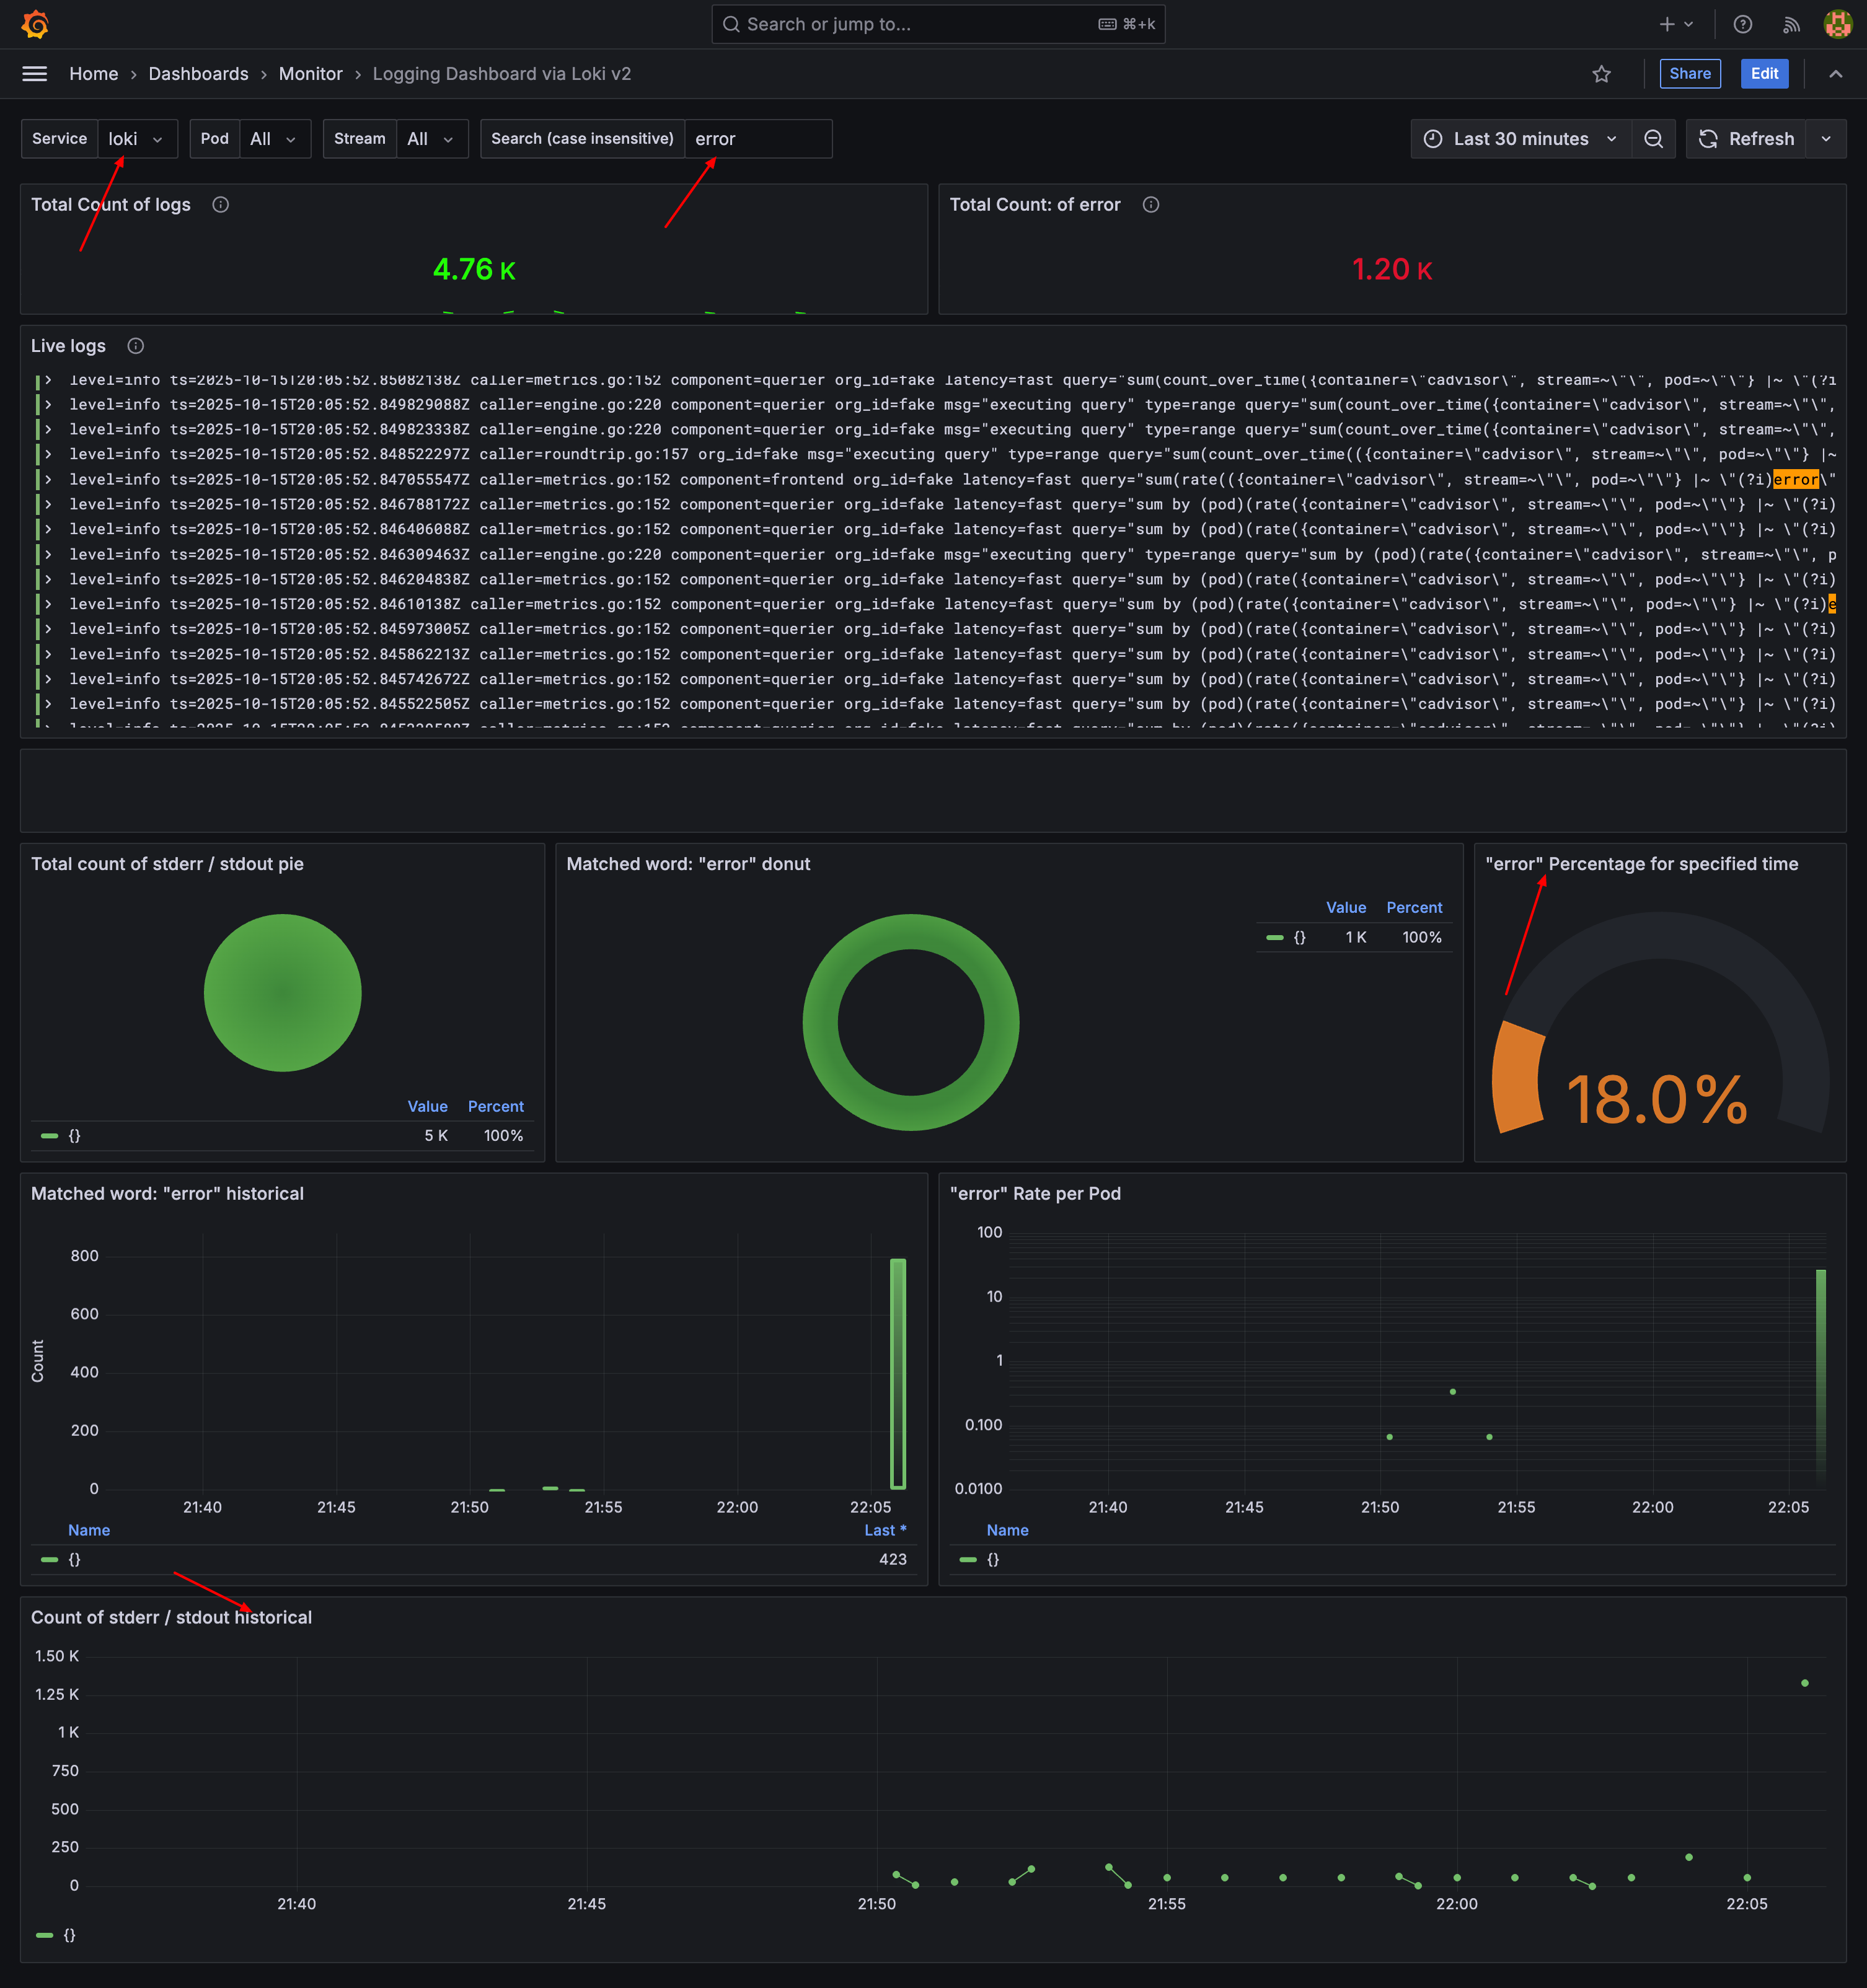
\includegraphics[width=16cm]{report/img/dashboard-aggregate-logging.png}
    \caption{}
    \label{log_aggregation}
\end{figure}

\newpage
\subsection{Log Tracing}

 \begin{figure}[!htb]
    \centering 
    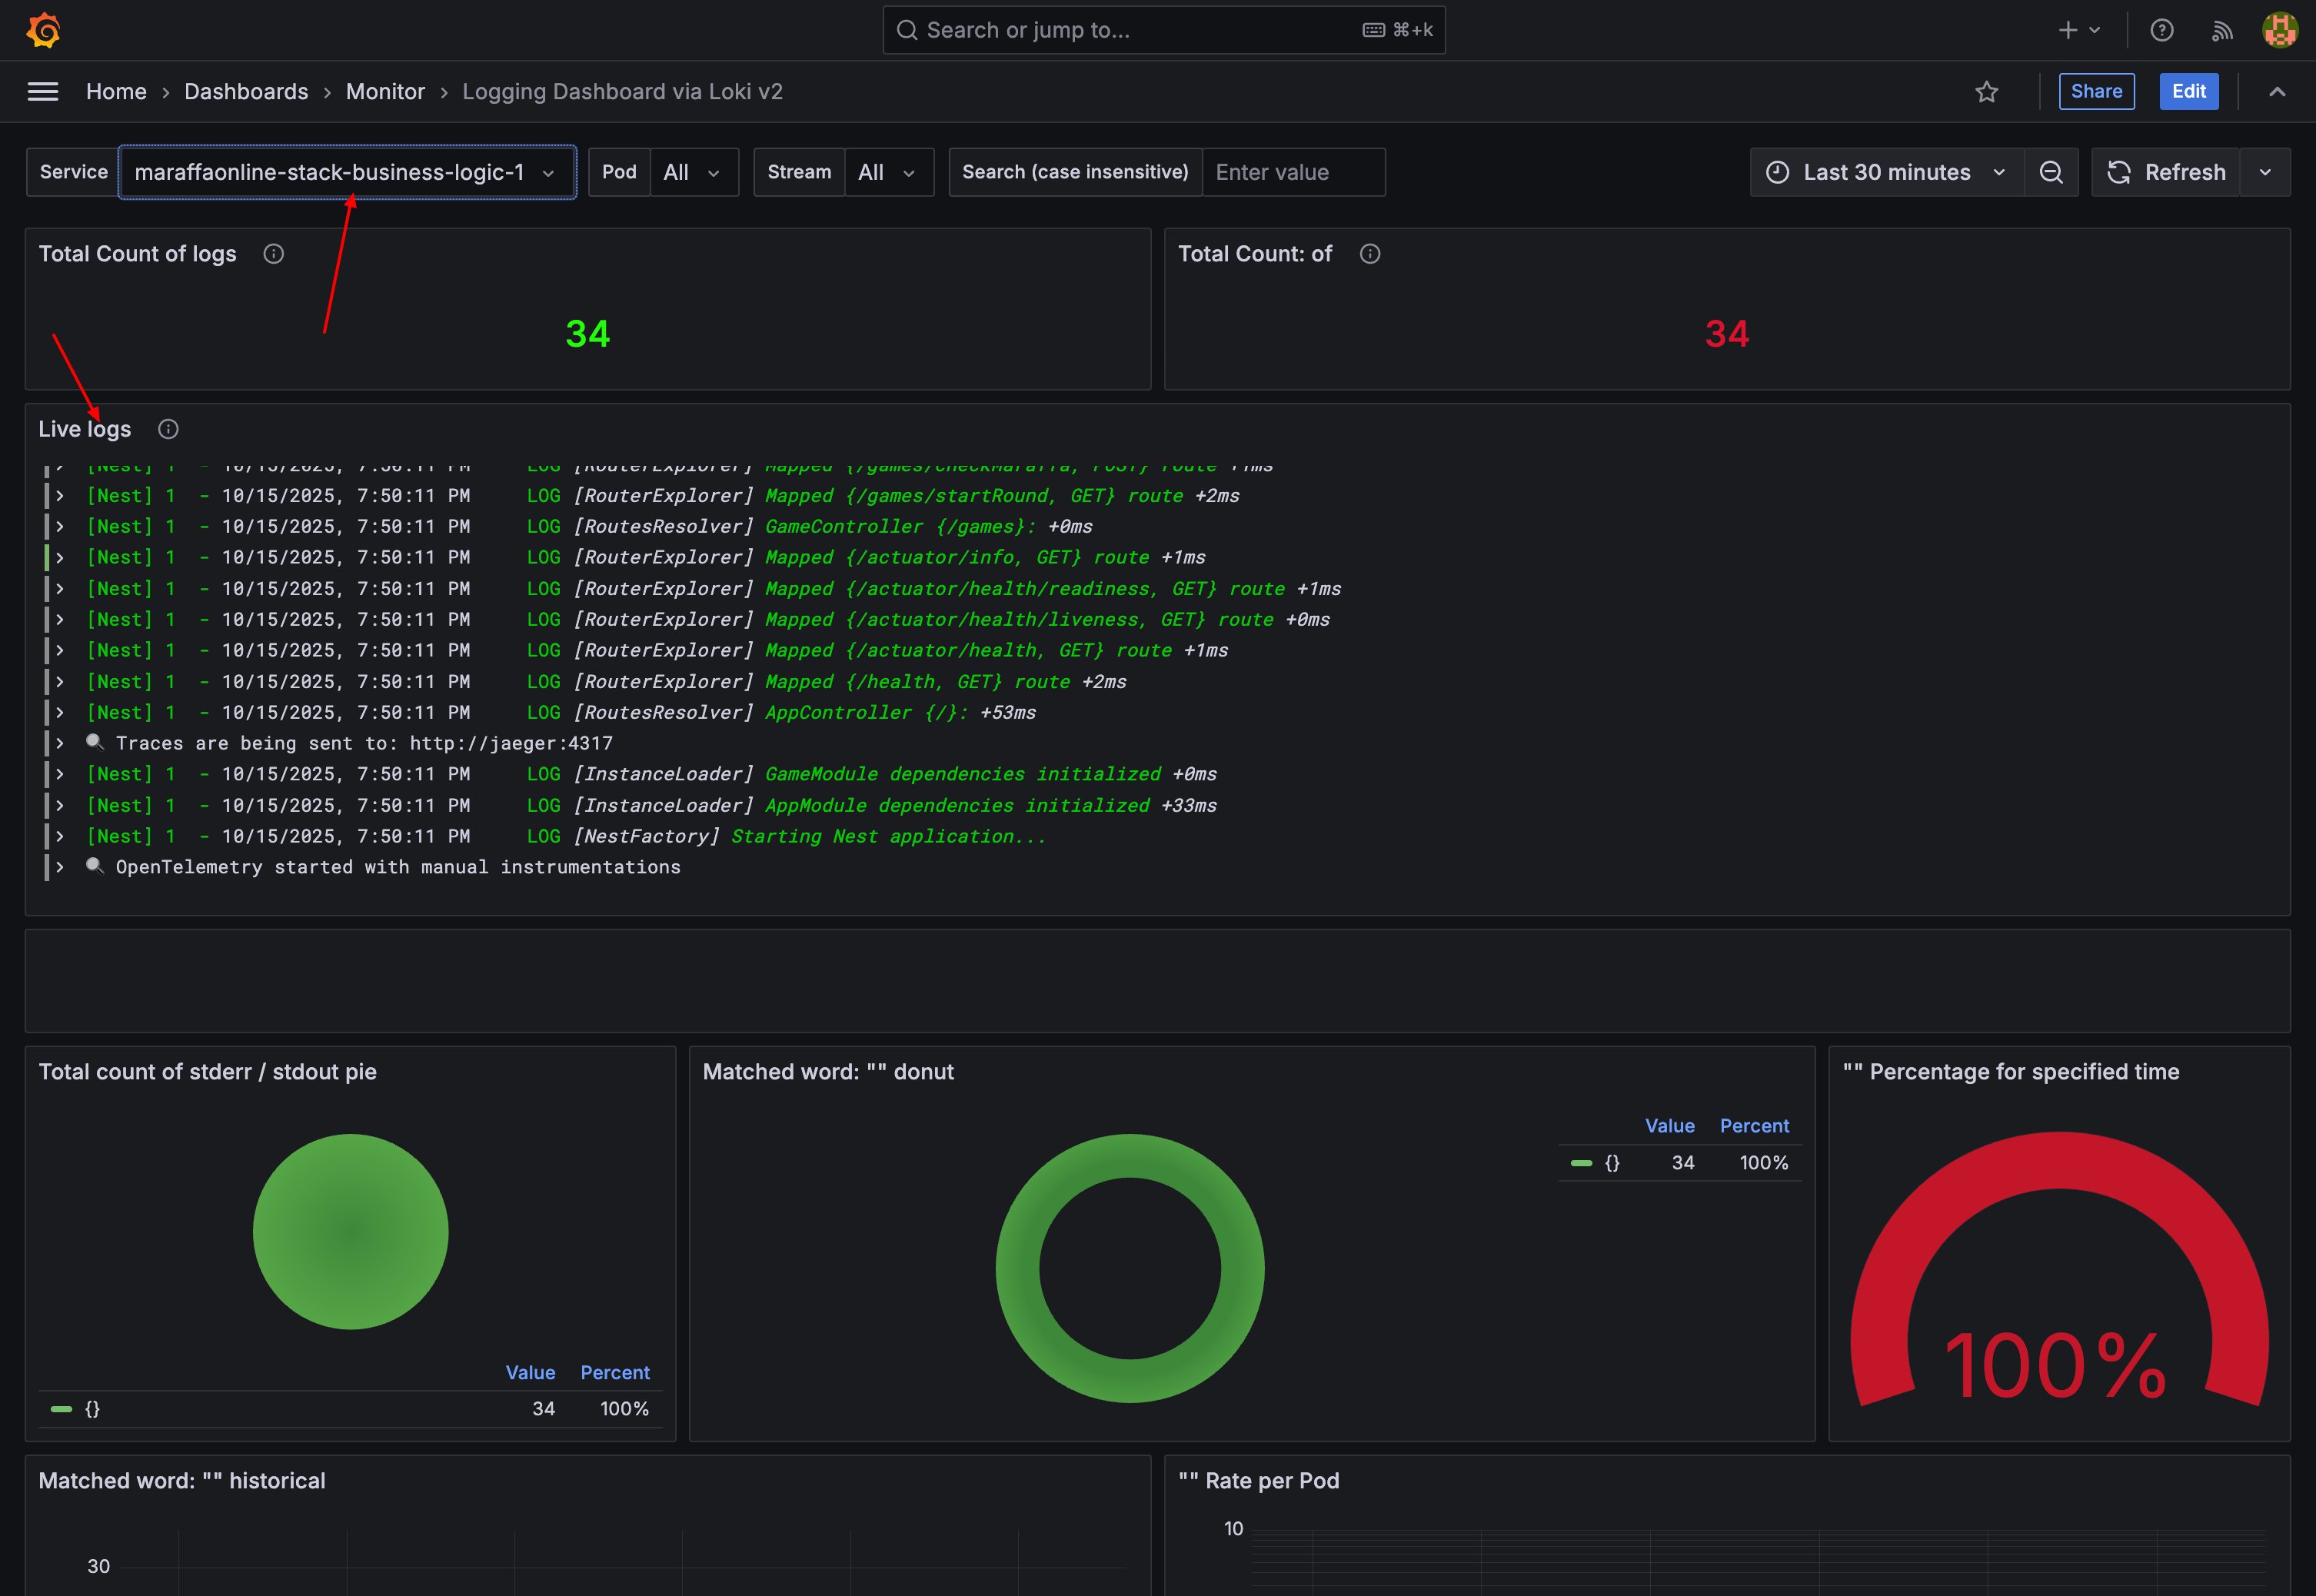
\includegraphics[width=16cm]{report/img/logging-service.png}
    \caption{}
    \label{log_tracing}
\end{figure}

\newpage
\subsection{Tracing servizi}

\begin{figure}[!htb]
    \centering 
    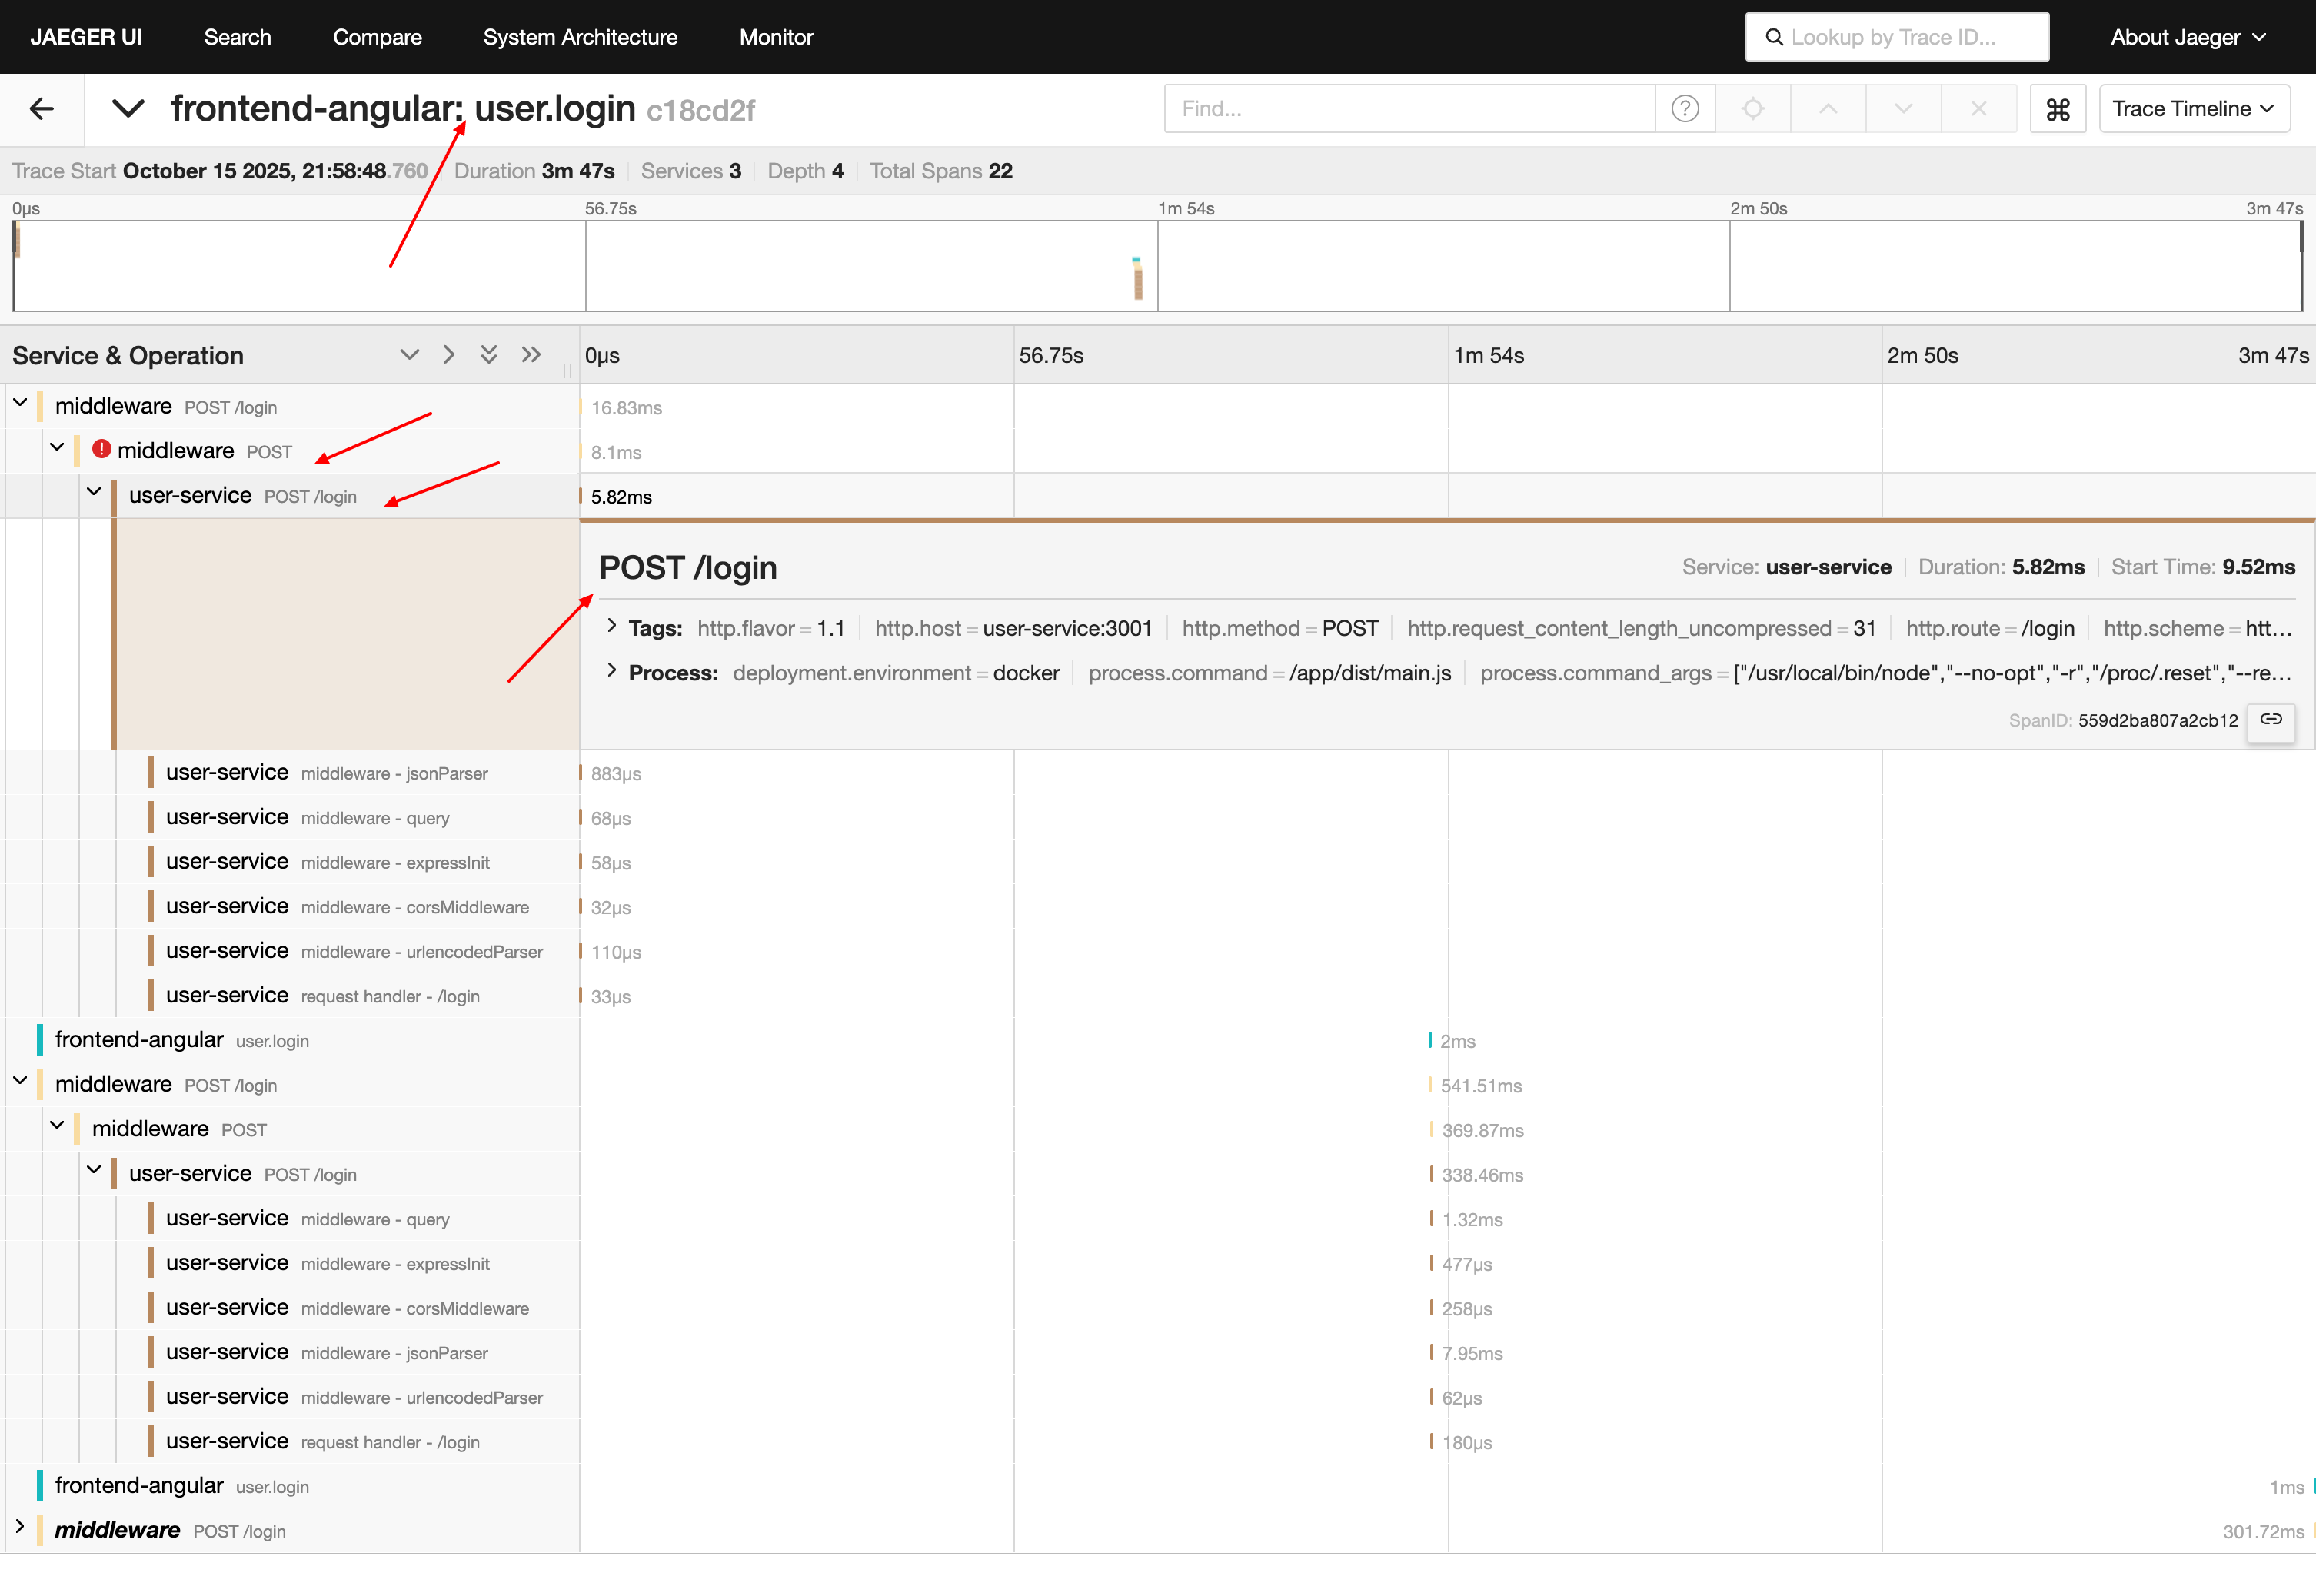
\includegraphics[width=16cm]{report/img/Jaeger-UI.png}
    \caption{}
    \label{service_tracing}
\end{figure}
\newpage